\documentclass{beamer}

\usepackage[utf8]{inputenc}
\usepackage[russian]{babel}
\usepackage{cmap}

\mode<presentation> {
\usetheme{Madrid}
\setbeamertemplate{caption}[numbered]
}

\usepackage{graphicx} % Allows including images
\usepackage{booktabs} % Allows the use of \toprule, \midrule and \bottomrule in tables

\title[Теория распознавания образов]{Локализация и отслеживание лиц на изображении}

\author{Мартынов Семён}
\institute[СП ПУ]
{
Санкт-Петербургский политехнический университет Петра Великогот \\
\medskip
\textit{semen.martynov@gmail.com}
}
\date{\today}

\begin{document}

\begin{frame}
\titlepage
\end{frame}

\begin{frame}
\frametitle{Содержание}
\tableofcontents
\end{frame}

%------------------------------------------------
\section{Базовые понятия}
%------------------------------------------------

\begin{frame}
\frametitle{Базовые понятия}
\begin{block}{Обнаружение лица}
Технология, определяющая наличие (иногда количество) лиц на цифровом изображении.
\end{block}

\begin{block}{Локализация лица}
Технология, определяющая положение лица на цифровом изображении (участке изображения), заведомо содержащем ровно одно лицо.
\end{block}

\begin{block}{Отслеживание лица}
Технология, определяющая положение лица в текущем кадре видео, и его смещение относительно предыдущего кадра.
\end{block}
\end{frame}

%------------------------------------------------

\begin{frame}
\frametitle{Пример автоматического обнаружения лиц}

\begin{figure}
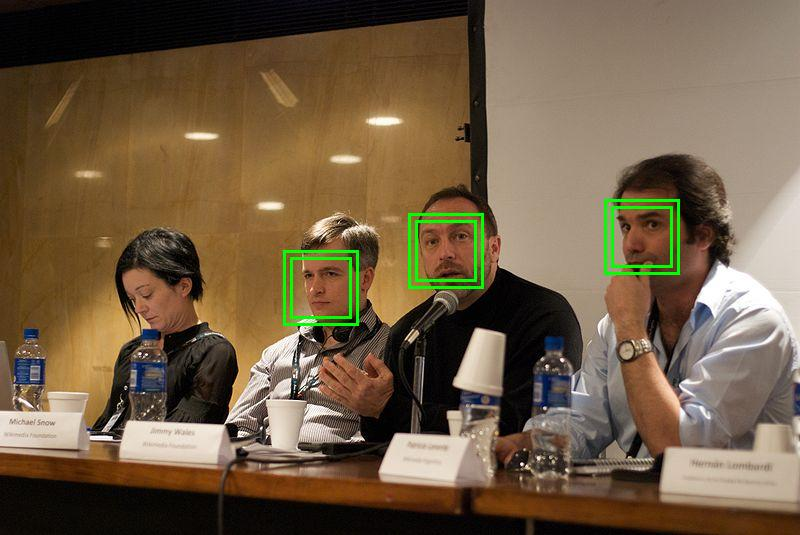
\includegraphics[scale=0.35]{res/img01}
\caption{Автоматическое обнаружение лиц при помощи OpenCV}
\end{figure}
\end{frame}

%------------------------------------------------
\section{Основы распознавания лиц}
%------------------------------------------------

\begin{frame}
\frametitle{Задачи обнаружения и распознавания лиц}

\begin{enumerate}
\item Задача обнаружения лиц (face detection)
    \begin{itemize}
    \item Охранные системы
    \item Автофокусировка
    \item Содержательная индексация базы изображений
    \end{itemize}
\pause
\item Задача распознавания лиц (Face Recognition)
    \begin{itemize}
    \item "Умные" охранные системы
    \item MOOC (Coursera)
    \item Верификация кредитных карточек
    \item Криминалистическая экспертиза
    \item Телеконференции
    \item Интерфейс человек-компьютер (Пример: SAMSUNG)
    \end{itemize}
\end{enumerate}
\end{frame}

%------------------------------------------------

\begin{frame}
\frametitle{Классы систем обнаружения лиц}

\begin{enumerate}
\item ручная - требует наличия оператора (офицер пограничной службы сравнивает фотографии из паспорта и реальное изображение человека);
\item автоматизированная - требует наличие оператора (доступ на охраняемый объект осуществляется по фотографии в документах и проксимити-карте);
\item автоматическая (задача установления личности осуществляется без участия человека).
\end{enumerate}
\end{frame}

%------------------------------------------------

\begin{frame}
\frametitle{Сложности построения автоматической системы}

\begin{enumerate}
\item сильно варьирующийся внешний вид лица у разных людей;
\item небольшое изменение ориентации лица относительно камеры приводит к серьезным изменениям изображения лица;
\item возможное присутствие индивидуальных особенностей (усы, бороды, очки, морщины и так далее);
\item изменение выражения лица (шум от эмоций);
\item часть лица может быть невидима (закрыта другими предметами) на изображении;
\item условия съемки (освещение, цветовой баланс камеры, искажения изображения, привносимые оптикой системы, качество изображения). 
\end{enumerate}
\end{frame}

%------------------------------------------------
\section{Эмпирические алгоритмы распознавания лиц}
%------------------------------------------------

\begin{frame}
\frametitle{Эмпирические алгоритмы распознавания лиц}

Основная идея - повторить работу человеческого мозга.

\begin{enumerate}
\item распознавание сверху-вниз -- принцип шаблона (производится описание свойств различных областей лица и их возможного взаимного расположения, а потом осуществляется проверка каждой из областей изображения на соответствие заданному шаблону);
\item Распознавание снизу-вверх -- инвариантные свойства (обнаружение и анализ элементов, инвариантных относительно условий съемки, которые характерны для изображения лица);
\end{enumerate}

\end{frame}

%------------------------------------------------
\subsection{Обнаружение характерных элементов и особенностей (features)}
%------------------------------------------------

\begin{frame}
\frametitle{Обнаружение характерных элементов и особенностей\\(features)}

\begin{itemize}
    \item \textbf{Края (edges)} -- резкие переходы яркости. Края обычно соответствуют границам объектов на изображении.
    \item \textbf{Яркость}. Области изображения, соответствующие чертам лица, зачастую темнее, чем окружающая их кожа.
    \item \textbf{Цвет} - цвет кожи разных людей занимает достаточно небольшую ограниченную подобласть цветового пространства (даже при рассмотрении цветов кожи различных рас)
    \item \textbf{Характерная форма черт лица} -- использование жестких или деформируемых шаблонов для обнаружения черт лица (например, глаз). 
\end{itemize}

\end{frame}
%------------------------------------------------
\begin{frame}
\frametitle{Обнаружение характерных элементов и особенностей\\(features)}

\begin{figure}
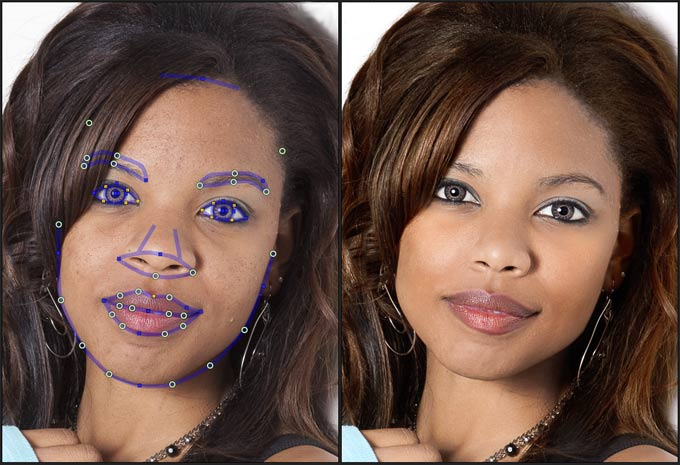
\includegraphics[scale=0.35]{res/img02}
\caption{Использование шаблонов для обнаружения черт лица}
\end{figure}

\end{frame}

%------------------------------------------------
\subsection{Комплексная проверка (complex test)}
%------------------------------------------------

\begin{frame}
\frametitle{Комплексная проверка\\(complex test)}

Основная идея в том, что обнаруживать элементы (глаза, нос, рот) легче, чем всё лицо. После этого нужно провести анализ их взаимного расположения с целью определения, могут ли они образовывать человеческое лицо.
\bigskip

Проверка соотношения обнаруженных признаков лица может быть основана на статистике взаимного расположения признаков.

\end{frame}
%------------------------------------------------
\begin{frame}
\frametitle{Комплексная проверка\\(complex test)}

\begin{figure}
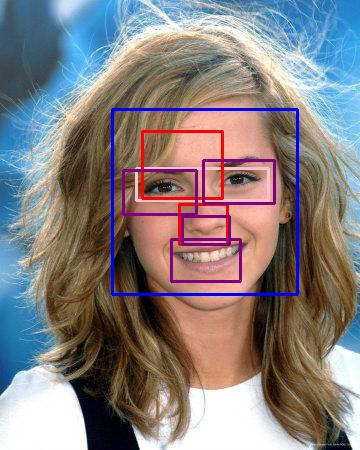
\includegraphics[scale=0.55]{res/img03}
\caption{Анализ взаимного расположения элементов лица}
\end{figure}

\end{frame}

%------------------------------------------------
\section{Алгоритмы математической статистики и машинного обучения}
%------------------------------------------------

\begin{frame}
\frametitle{Алгоритмы математической статистики\\и машинного обучения}

\end{frame}

%------------------------------------------------
\subsection{Метод Главных Компонент (PCA)}
%----------------------------------------------

\begin{frame}
\frametitle{Метод Главных Компонент\\(Principal Components Analysis, PCA)}

\end{frame}

%------------------------------------------------
\subsection{Факторный анализ (FA)}
%----------------------------------------------

\begin{frame}
\frametitle{Факторный анализ\\(Factor Analysis, FA)}

\end{frame}

%------------------------------------------------
\subsection{Смесь многомерных нормальных распределений (MoG)}
%----------------------------------------------

\begin{frame}
\frametitle{Смесь многомерных нормальных распределений\\(mixture of Gaussians, MoG)}

\end{frame}

%------------------------------------------------
\subsection{Линейный Дискриминантный Анализ (LDA)}
%----------------------------------------------

\begin{frame}
\frametitle{Линейный Дискриминантный Анализ\\(Linear Discriminant Analysis, LDA)}

\end{frame}

%------------------------------------------------
\subsection{Метод Опорных Векторов (SVM)}
%----------------------------------------------

\begin{frame}
\frametitle{Метод Опорных Векторов\\(Support Vector Machines, SVM)}

\end{frame}

%------------------------------------------------
\subsection{Искусственные Нейронные Сети (NN)}
%----------------------------------------------

\begin{frame}
\frametitle{Искусственные Нейронные Сети\\(Neural Networks, NN)}

\end{frame}

%------------------------------------------------
\subsection{Разреженная сеть просеивающих элементов (SNoW)}
%----------------------------------------------

\begin{frame}
\frametitle{Разреженная сеть просеивающих элементов\\(Sparse Network of Winnows, SNoW)}

\end{frame}

%------------------------------------------------
\subsection{Скрытые Марковские Модели (HMM)}
%----------------------------------------------

\begin{frame}
\frametitle{Скрытые Марковские Модели\\(Hidden Markov Models, HMM)}

\end{frame}

%------------------------------------------------
\subsection{Активные модели внешнего вида (AAM)}
%----------------------------------------------

\begin{frame}
\frametitle{Активные модели внешнего вида\\(Active Appearance Models, AAM)}

\end{frame}

%------------------------------------------------
\section{Вопросы}
%------------------------------------------------

\begin{frame}
\Huge{\centerline{Вопросы?}}
\end{frame}

%----------------------------------------------------------------------------------------

\end{document} 